\documentclass[10pt,journal,compsoc]{IEEEtran}

\usepackage[utf8]{inputenc}
\usepackage[T1]{fontenc}
\usepackage{amsmath,amssymb,amsfonts}
\usepackage{graphicx}
\usepackage{booktabs}
\usepackage{multirow}
\usepackage{array}
\usepackage{microtype}
\usepackage{hyperref}
\usepackage{cleveref}
\usepackage{xcolor}
\usepackage{listings}

\hypersetup{
    colorlinks=true,
    linkcolor=blue!70!black,
    citecolor=blue!70!black,
    urlcolor=blue!70!black
}

\lstset{
    basicstyle=\ttfamily\footnotesize,
    breaklines=true,
    frame=single,
    backgroundcolor=\color{gray!10},
    numbers=left,
    numberstyle=\tiny\color{gray},
    keywordstyle=\color{blue!80!black}\bfseries,
    commentstyle=\color{green!50!black}\itshape,
    stringstyle=\color{red!70!black}
}

\begin{document}

\title{FinLens: A Robust Text-to-Pandas Architecture with Concept Coverage Table Selection and AST-Governed Sandboxed Execution for Financial Statement Question Answering}

\author{FinLens AI Research Team}

\markboth{FinLens Technical Architecture Documentation}%
{FinLens Technical Architecture Documentation}

\IEEEtitleabstractindextext{%
\begin{abstract}
Answering numerical questions over corporate financial statements involves document retrieval, table selection, accounting unit handling, and numerical calculation. FinLens is a Text to Pandas system developed for this task. Its online pipeline combines metadata parsing, dense and lexical retrieval, cross encoder reranking, table selection with concept coverage checks, context planning, Pandas code generation, static code validation, and execution in an isolated E2B sandbox. When the pipeline produces a valid answer, it also records the supporting document, table, CSV file, and Pandas query. This paper describes the product architecture, the ViFinQA data used by the system, the data preparation process, and the available benchmark results.
\end{abstract}

\begin{IEEEkeywords}
Financial Question Answering, Text-to-Pandas, Table Retrieval, Cross-Encoder Reranking, Concept Coverage Matrix, AST Code Validation, Sandboxed Execution.
\end{IEEEkeywords}}

\maketitle

\IEEEdisplaynontitleabstractindextext
\IEEEpeerreviewmaketitle

\section{Introduction}
\IEEEPARstart{Q}{uestion} answering over corporate financial statements combines document understanding, table retrieval, and numerical reasoning~\cite{chen2021finqa,zhu2021tat,islam2023financebench}. Financial questions may require several calculation steps and may depend on reporting scope, accounting units, and the structure of each report. Example tasks include calculating ratios, comparing values across companies, and distinguishing consolidated reports from separate reports.

Solving these questions presents three practical challenges:
\begin{enumerate}
    \item \textbf{Schema Heterogeneity \& Extraction Noise}: Corporate filings extracted from scanned PDF or HTML documents exhibit varying row label depths, note references, unit scales (e.g., raw currency vs. millions vs. billions), and non-standard tabular structures that resist rigid SQL schema assumptions.
    \item \textbf{Computational Completeness vs. Semantic Similarity}: Standard dense retrievers and cross-encoders optimize for textual relevance rather than mathematical sufficiency. A financial calculation such as $R = \frac{\text{Current Assets}}{\text{Current Liabilities}}$ requires \textit{both} accounting concepts; returning multiple redundant asset tables while omitting liabilities results in computational failure.
    \item \textbf{Code Generation Vulnerabilities}: Directly executing LLM-generated Python/Pandas logic can introduce silent precision drift from unrequested rounding, ungrounded access to metadata properties, and hazardous host execution environments~\cite{gao2023pal,chen2023pot,agache2020firecracker}.
\end{enumerate}

FinLens addresses these challenges by combining language model components with deterministic validation and execution steps. The following sections describe the system architecture, data preparation pipeline, and available evaluation results.

\begin{figure*}[!t]
\centering
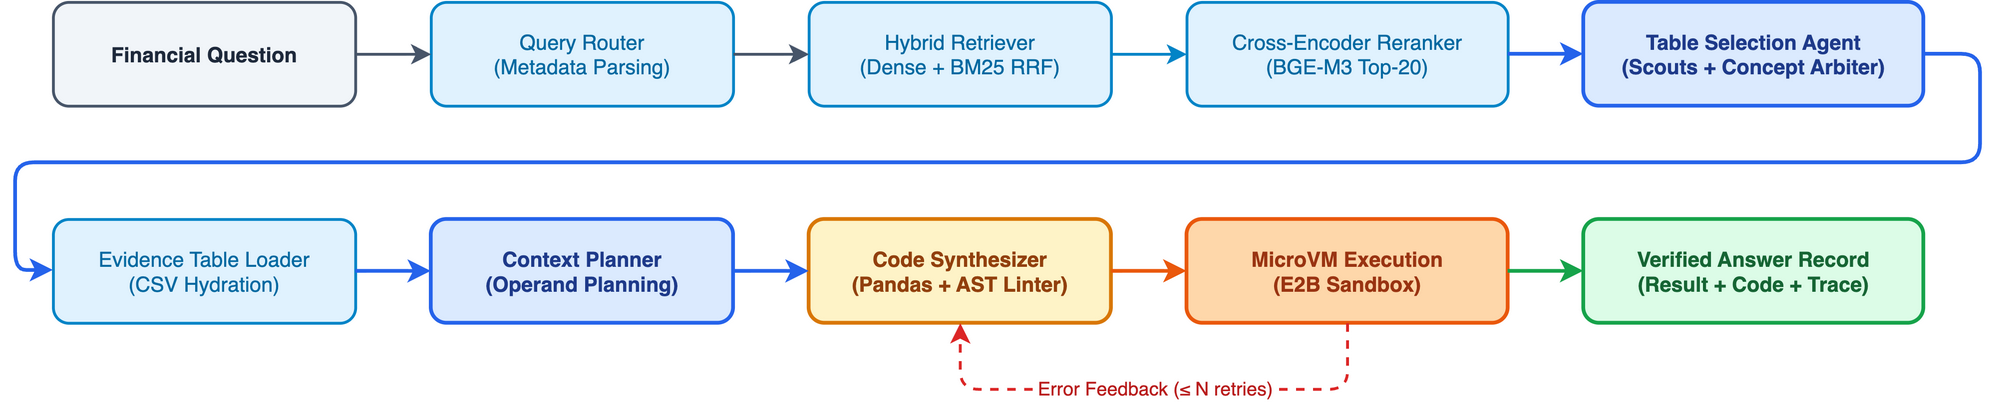
\includegraphics[width=0.98\textwidth]{figures/system_topology.png}
\caption{\textbf{FinLens System Topology.} The online pipeline moves from question parsing and hybrid retrieval to cross encoder reranking, table selection, context planning, code generation, validation, and execution in an E2B sandbox. A successful run produces an answer record with its supporting references.}
\label{fig:system_topology}
\end{figure*}

\section{System Architecture \& Online Inference}
The FinLens online execution pipeline is implemented as a LangGraph state graph. A typed state container $\mathcal{S}$ (\texttt{RetrievalState}) carries the canonical question $q$, metadata filters $\mathcal{F}$, candidate tables, loaded DataFrames $\mathcal{D}$, planning context $\mathcal{P}$, generated code $\mathcal{C}$, attempt counters, and execution feedback.

As shown in \Cref{fig:system_topology}, the architecture separates language model calls from deterministic processing and execution steps:
\begin{equation}
\begin{aligned}
    q &\xrightarrow{\text{Upstream}} \mathcal{T}_{80} \xrightarrow{\text{Rerank}} \mathcal{T}_{20} \xrightarrow{\text{Select}} \mathcal{T}^* \\
      &\xrightarrow{\text{Load}} \mathcal{D} \xrightarrow{\text{Plan}} \mathcal{P} \xrightarrow{\text{Synthesize}} \mathcal{C} \underset{\text{Retry}}{\overset{\text{Execute}}{\rightleftharpoons}} \mathcal{A}
\end{aligned}
\end{equation}
where $\mathcal{T}_{80}$ represents the candidates from hybrid retrieval, $\mathcal{T}_{20}$ denotes the cross encoder reranked subset, $\mathcal{T}^*$ represents the tables selected for calculation, $\mathcal{D}$ denotes the loaded DataFrames, $\mathcal{P}$ is the planning context, $\mathcal{C}$ is the validated Python script, and $\mathcal{A}$ is the final answer record.

\subsection{Query Routing \& Hybrid Retrieval}
Incoming queries are processed by a Query Router Agent that validates ticker symbols, reporting years (restricted to the canonical 2015--2025 window), and disclosure scopes (\textit{consolidated}, \textit{separate}, \textit{aggregated}). Candidate tables are retrieved using a hybrid strategy combining dense embedding search with BM25 lexical matching via Reciprocal Rank Fusion (RRF)~\cite{cormack2009reciprocal,robertson2009probabilistic} to produce a balanced pool of up to 80 candidate tables $\mathcal{T}_{80}$.

\subsection{Cross-Encoder Reranking \& Context Packaging}
To refine the initial candidate pool, FinLens deploys a multilingual cross-encoder reranker based on BGE-M3~\cite{chen2024bge}. Because full tabular CSVs exceed standard token windows, FinLens builds a layered contextual representation for each candidate table:
\begin{itemize}
    \item \textbf{Structural Header \& Metadata}: Extracted titles, reporting years, and column names.
    \item \textbf{Complete Row Catalog}: A lightweight index mapping all row indices to standardized accounting line codes and normalized labels without truncation.
    \item \textbf{Lexical Seed \& Neighbor Expansion}: Seed rows matching question tokens are expanded with immediate vertical neighbors $(r-1, r, r+1)$ to preserve subtotals and subsection hierarchy.
    \item \textbf{Bounded Serialization}: High-signal match summaries are packed into a bounded document ($\le 6,000$ characters) for cross-encoder scoring, yielding the top 20 finalist tables ($\mathcal{T}_{20}$).
\end{itemize}

\begin{figure*}[!t]
\centering
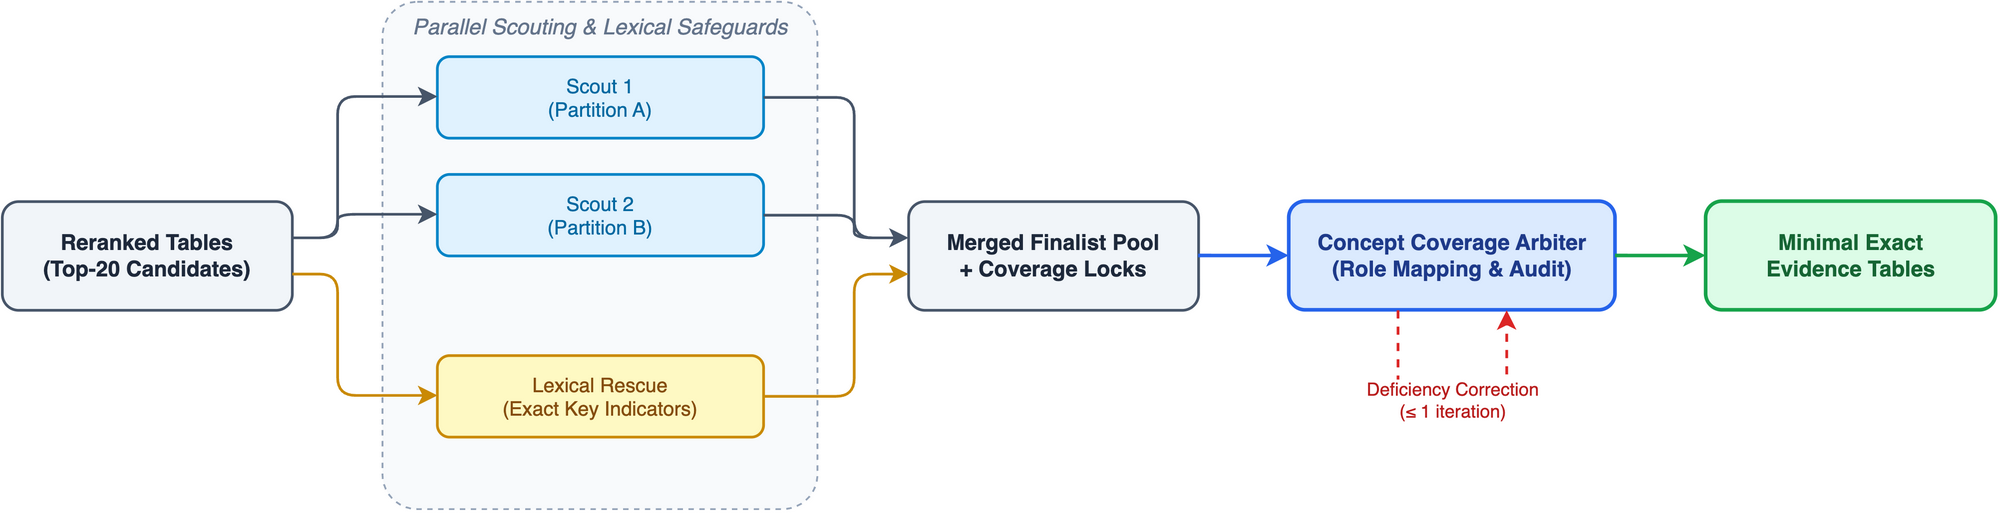
\includegraphics[width=0.95\textwidth]{figures/table_selection.png}
\caption{\textbf{Two Stage Table Selection Architecture.} Two scouts propose candidate tables and a lexical check retains tables that contain exact indicator phrases. The final selector checks whether the proposed tables cover the accounting concepts identified in the question.}
\label{fig:table_selection}
\end{figure*}

\subsection{Two-Stage Table Selection with Concept Coverage}
FinLens uses a two stage table selection process with concept coverage checks (\Cref{fig:table_selection}):
\begin{enumerate}
    \item \textbf{Parallel Scouting}: The 20 candidates are partitioned into balanced chunks across document buckets (ticker and year pairs), and two parallel LLM scouts nominate all candidates capable of providing at least one required operand.
    \item \textbf{Lexical Rescue}: An out-of-band filter bypasses scout pruning for candidates containing exact multi-word indicator phrases from the question.
    \item \textbf{Concept Coverage Arbiter}: The arbiter decomposes the question into financial concepts with explicit computational roles $\rho \in \mathcal{R}_{\text{roles}}$:
    \begin{equation}
        \mathcal{R}_{\text{roles}} = \left\{
        \begin{array}{l}
            \text{direct}, \, \text{numerator}, \, \text{denominator}, \\
            \text{beginning\_balance}, \, \text{ending\_balance}, \\
            \text{comparison\_operand}
        \end{array}
        \right\}
    \end{equation}
    The selector maps each identified concept to a candidate table. Local checks look for uncovered concepts, selected tables without a mapped concept, and required comparison groups that are not represented. If the response does not satisfy these checks, the system requests one corrected selector response.
\end{enumerate}

\subsection{Grounded Planning \& Dynamic Row Hydration}
Approved tables $\mathcal{T}^*$ are loaded into memory as isolated DataFrames $\mathcal{D} = \{ \text{df}_1: \mathbf{D}_1, \dots, \text{df}_m: \mathbf{D}_m \}$. A Planning Agent generates a four-field structured plan (\textit{evidence}, \textit{calculation}, \textit{unit\_conversion}, \textit{audit}) declaring exact row positions and operational purposes. If catalog rows outside the initial detailed preview are referenced, FinLens dynamically \textit{hydrates} their full numerical values from disk on demand, ensuring complete data access without prompt bloat.

\begin{figure*}[!t]
\centering
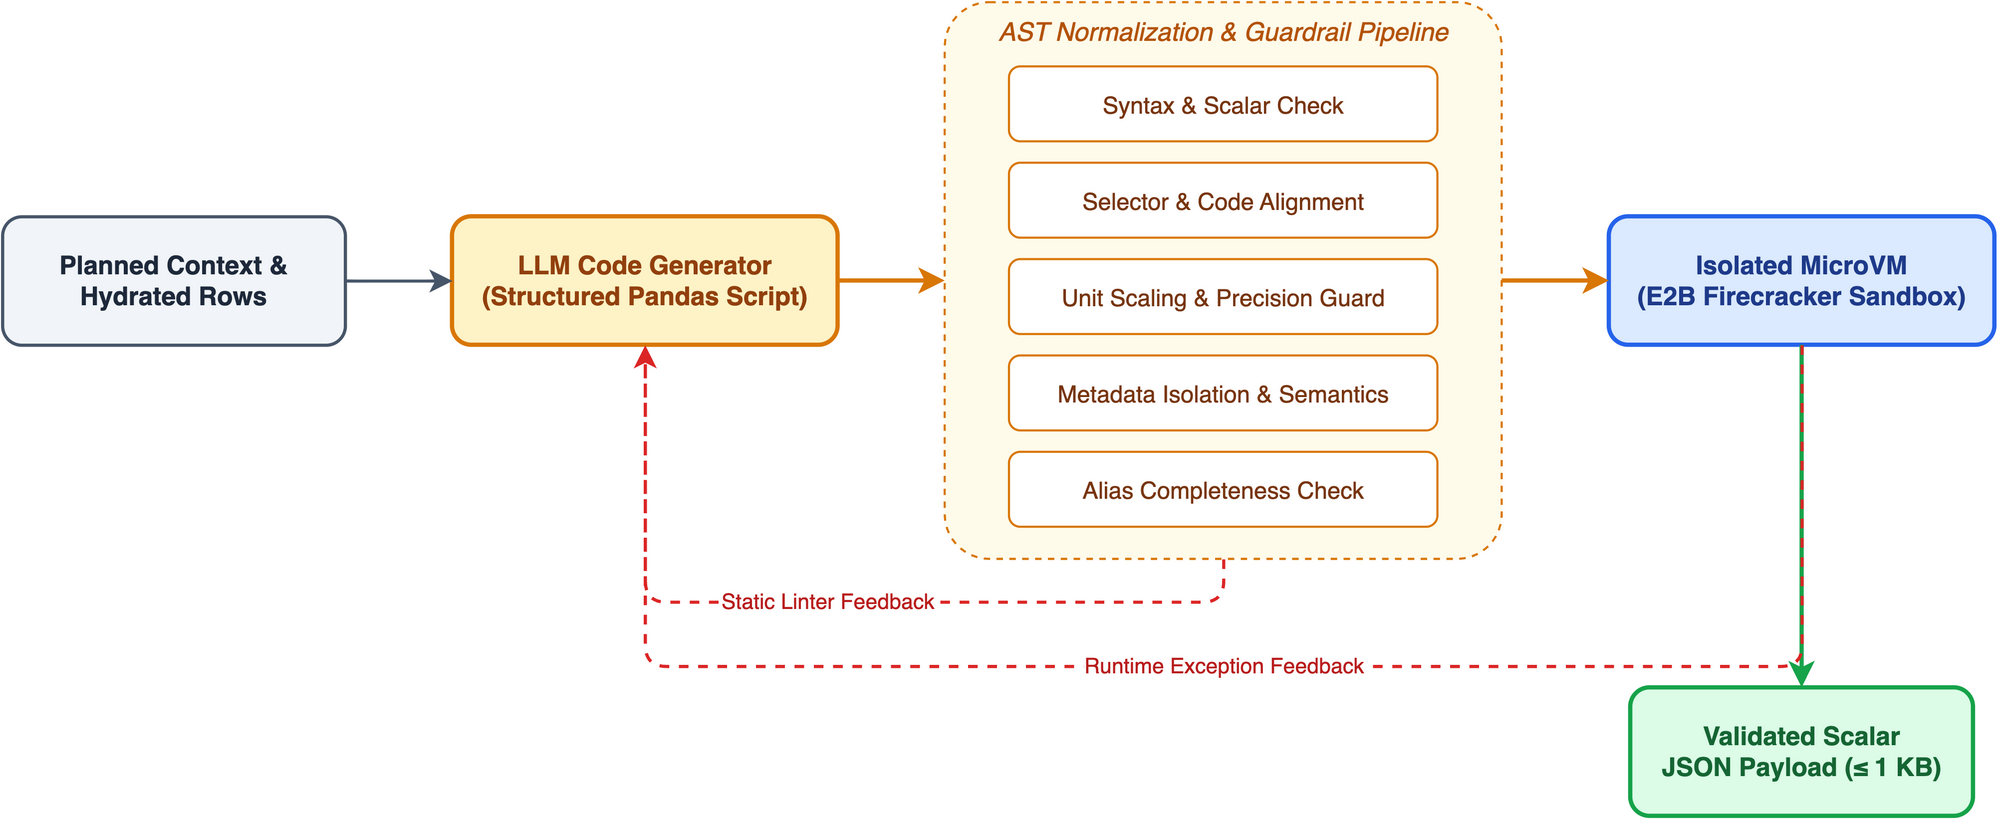
\includegraphics[width=0.95\textwidth]{figures/synthesis_and_sandbox.png}
\caption{\textbf{Code Validation and Sandboxed Execution Workflow.} Generated Pandas code passes through static syntax, selector, unit, precision, and access checks before execution in an isolated E2B sandbox. Validation and execution errors are returned to the generator within a limited retry loop.}
\label{fig:synthesis_and_sandbox}
\end{figure*}

\subsection{AST-Governed Code Synthesis \& Multi-Pass Guardrails}
The Code Synthesis Agent emits structured Python/Pandas logic $\mathcal{C}_{\text{raw}} = \{ \text{"pandas\_query"}: \text{str}, \, \text{"evidence\_variables"}: [\text{str}] \}$. Before execution, the code is parsed into an Abstract Syntax Tree (AST) and processed through an 8-pass normalization pipeline (\Cref{tab:ast_passes} and \Cref{fig:synthesis_and_sandbox}):
\begin{itemize}
    \item \textbf{Syntax \& Scalar Normalization}: Enforces parseable Python syntax and automatic assignment of the final scalar to \texttt{result}.
    \item \textbf{Selector \& Unit Alignment}: Canonicalizes boolean filter literals (e.g., \texttt{'10.0'} $\rightarrow$ \texttt{'10'}) and automatically normalizes currency divisors ($10^6, 10^9, 10^{12}$) based on cell magnitudes.
    \item \textbf{Access \& Precision Checks}: Rejects rounding that was not requested, access to unsupported DataFrame metadata attributes (\texttt{df.metadata} / \texttt{df.attrs}), and generated calculations that do not contain expected operations for selected question types.
\end{itemize}

\begin{table*}[!t]
\centering
\caption{FinLens Multi-Pass AST Validation and Normalization Pipeline}
\label{tab:ast_passes}
\begin{tabular}{lllp{7.5cm}}
\toprule
\textbf{Pass} & \textbf{Validation Target} & \textbf{Action Type} & \textbf{Description \& Architectural Enforcement} \\
\midrule
1 & Syntax \& Envelope & Validation & Verifies parseable Python syntax and presence of required schema fields. \\
2 & Scalar Assignment & Normalization & Ensures final value is assigned to \texttt{result}; converts bare trailing expressions to \texttt{result = expr}. \\
3 & Name Resolution & Validation & Scans \texttt{ast.Load} nodes and reports local names that are not defined before runtime. \\
4 & Selector Alignment & Normalization / Rejection & Canonicalizes string and code filters against loaded DataFrame values; suggests valid context values on mismatch. \\
5 & Unit Scale Normalizer & Normalization / Rejection & Aligns question currency units with cell magnitudes ($>10^{10}$ vs. $<10^9$); automatically inserts or corrects scale divisors. \\
6 & Precision Guard & Rejection & Prohibits intermediate \texttt{.round()} calls unless the natural language question explicitly mandates rounding. \\
7 & Metadata Isolation & Rejection & Traces variable assignments and rejects access to \texttt{df.metadata} or \texttt{df.attrs}. \\
8 & Domain Semantics & Rejection & Checks for percentage conversion, subtraction in selected growth or difference questions, and use of the aliases selected for the calculation. \\
\bottomrule
\end{tabular}
\end{table*}

\subsection{Sandboxed MicroVM Execution \& Dual-Layer Retries}
Validated code is executed inside ephemeral Firecracker microVMs managed via E2B~\cite{agache2020firecracker}, with network access disabled (\texttt{allow\_internet\_access = False}) and a 5.0-second execution timeout. Results are extracted through a bounded two-step serialization protocol writing a verified scalar JSON payload ($\le 1,024$ bytes) to disk.

The system incorporates a dual-layer fault-tolerance model:
\begin{enumerate}
    \item \textbf{Transient Retries}: Network and API hiccups are handled automatically by node-level retry policies without consuming semantic reasoning attempts.
    \item \textbf{Semantic Retries}: AST validation rejections and runtime microVM exceptions are converted into structured diagnostic feedback and routed back to the Code Synthesis Agent (up to a configurable attempt limit $1 \le \text{max\_attempts} \le 5$).
\end{enumerate}

\subsection{Answer Provenance Assembly}
Upon successful execution, FinLens creates an \texttt{answer\_record} that stores the numeric answer, the document ID, the table start line, the CSV path, and the Pandas query used for the calculation.

% =========================================================================
% SECTION 3: DATASET & DATA PROCESSING PIPELINE (COLLABORATOR SECTION)
% =========================================================================
\section{Dataset \& Data Processing Pipeline}
\subsection{Dataset Source and Scope}
FinLens uses the \textbf{ViFinQA} dataset released by AIGuruTinix on Hugging Face~\cite{aigurutunix2026vifinqa}. The dataset contains Vietnamese questions and financial reports that have been converted into text by OCR. FinLens starts from these provided text files. It does not collect reports and it does not perform OCR.

Each question has an integer ID and a canonical question text. Each report is organized by ticker, year, and report scope. The report scope can be consolidated, separate, aggregated, or other. The current local data contains 1,012 questions and 1,973 reports from 100 stock tickers. The reports cover the period from 2015 to 2025.

\begin{table}[!t]
\centering
\caption{Current Local ViFinQA Data and Exported Table Counts}
\label{tab:dataset_stats}
\resizebox{\columnwidth}{!}{
\begin{tabular}{lrr}
\toprule
\textbf{Item} & \textbf{Value} & \textbf{Share} \\
\midrule
Questions & 1,012 & Not applicable \\
Stock tickers & 100 & Not applicable \\
Financial reports & 1,973 & Not applicable \\
Reporting period & 2015 to 2025 & Not applicable \\
Exported CSV tables & 144,406 & 100.0\% \\
\quad Balance sheets & 8,822 & 6.1\% \\
\quad Income statements & 5,677 & 3.9\% \\
\quad Cash flow statements & 4,235 & 2.9\% \\
\quad Note tables & 125,672 & 87.0\% \\
\bottomrule
\end{tabular}
}
\end{table}

\begin{figure*}[!t]
\centering
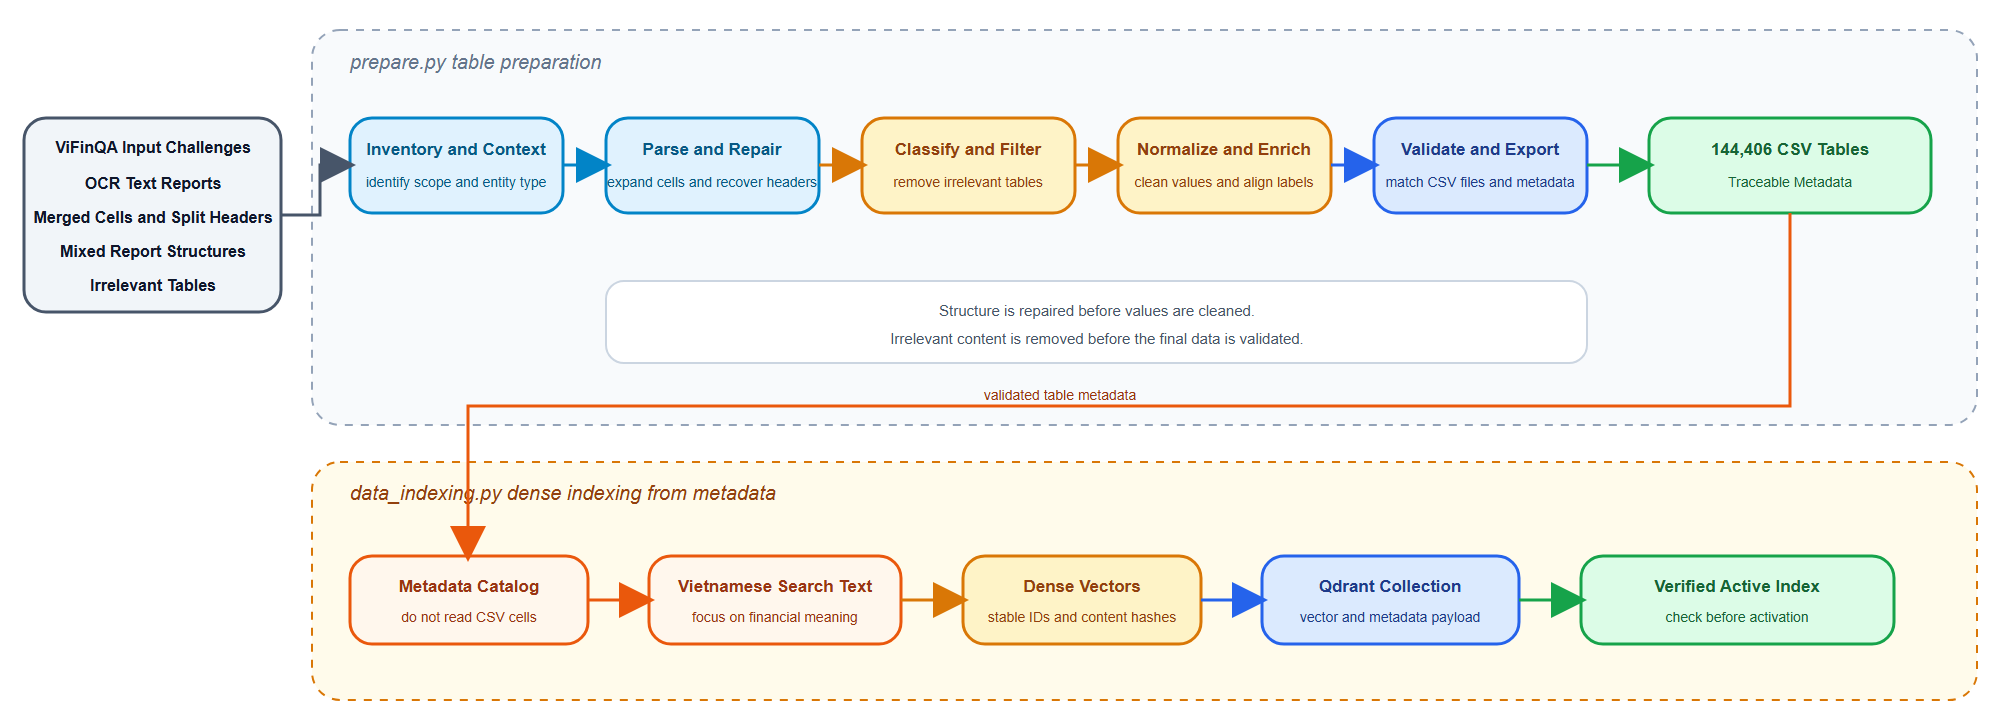
\includegraphics[width=0.98\textwidth]{figures/data_processing_pipeline.png}
\caption{\textbf{FinLens Data Processing Pipeline.} The upper path shows how the pipeline repairs structure, removes irrelevant content, improves consistency, and preserves traceability. The lower path builds and verifies a dense search index from metadata without embedding CSV cell contents.}
\label{fig:data_processing_pipeline}
\end{figure*}

\subsection{Data Characteristics and Challenges}
The OCR text contains HTML tables, but their structure is not always clean. Some tables contain merged rows or columns. Some headers are separated from the table body. These issues can move a value away from its correct financial indicator.

The reports also follow different structures. General enterprises, credit institutions, securities companies, and insurance companies use different report forms. The current data contains 74 general enterprise tickers, 22 credit institution tickers, 3 securities company tickers, and 1 insurance company ticker. Consolidated and separate reports can contain similar indicators with different meanings. The same indicator can also have different labels and units across companies and years.

Not every HTML table contains useful financial data. A table can be a table of contents, an administrative section, or an incomplete header. Note tables are especially varied and account for 87.0\% of all exported tables. If these issues are not handled, the system can index irrelevant content, connect a question to the wrong table, or lose the link to the source report.

\subsection{Data Preparation and Validation}
The preparation pipeline is shown in \Cref{fig:data_processing_pipeline}. It first records the ticker, year, report scope, document ID, file size, and page count. It also detects the entity type from report form codes and strong text clues. This context helps the next stages apply the correct rules to each report.

The parser then converts each HTML table into rows. It expands merged cells and recovers nearby header context when needed. At the same time, it keeps a stable table ID and the original starting line. This process repairs common table structures while preserving the path back to the source report.

The pipeline classifies each table by using report form codes, heading text, and table structure. It keeps balance sheets, income statements, cash flow statements, and note tables. It removes tables of contents, incomplete headers, and administrative content before export. It also cleans numeric cells and builds consistent Vietnamese labels from recurring item codes. These steps reduce irrelevant tables and make similar financial indicators easier to find.

Each accepted table is saved as a separate CSV file. The pipeline also creates document metadata, table metadata, semantic summaries, and keywords. A final validation checks that every table has one CSV file, one unique ID, a valid report scope, and a valid source line. Intermediate records keep the reason for every skipped table and every intentional repair. This makes the output consistent and traceable.

\subsection{Building the Search Index}
The indexing script reads the table metadata as a stream and creates a JSONL manifest. It does not read CSV cell contents at this stage. This choice keeps the index small and prevents noisy cell values from dominating the meaning of a table.

For each accepted table, the script creates short Vietnamese search text from the table type, semantic summary, indicator names, and keywords. Ticker, company name, year, and file path are kept as filters instead of being repeated in the search text. This separation helps the vector represent financial meaning while the filters preserve document identity.

The search text is converted into a dense vector and stored in Qdrant. The payload keeps the table ID, document ID, ticker, company name, year, report scope, table type, source line, and search text. Stable point IDs, content hashes, and a local SQLite checkpoint allow an interrupted upload to continue and prevent unchanged tables from being uploaded again.

After the upload, the script compares Qdrant with the manifest. It activates the new collection only when the counts and sampled records are correct. This check prevents an incomplete index from being used online. The stored index contains dense vectors. When hybrid retrieval is enabled, BM25 is calculated at query time over the filtered search text and is then combined with the dense results.

% =========================================================================
% SECTION 4: EXPERIMENTS & BENCHMARK EVALUATION (COLLABORATOR SECTION)
% =========================================================================
\section{Experiments \& Benchmark Evaluation}

\subsection{Experimental Setup}

The experiment uses all 1,012 questions in the ViFinQA evaluation set. The final submission and prediction archives contain the same 859 prediction records. Each record includes an answer, relevant documents, relevant tables, evidence, and a Pandas query. The remaining 153 questions do not have a prediction record. This gives a prediction coverage of 84.88\%.

The language model is Qwen 3.5 9B. In the environment file, \texttt{LLM\_MODEL} selects Qwen 3.5 9B, \texttt{LLM\_TEMPERATURE} is 0.1, and \texttt{LLM\_TIMEOUT} is 60 seconds. A low temperature makes numerical answers and generated queries more stable. The timeout prevents one difficult question from stopping the full evaluation process. Document and table retrieval use the IBM Granite multilingual embedding model with 97 million parameters, revision R2. The vectors are stored in the Qdrant collection selected by \texttt{QDRANT\_COLLECTION}.

The official scoring archive was produced successfully with exit code 0. Its scoring process took about 4.98 seconds. This time only describes the scoring step. It does not include document processing, retrieval, or model inference.

\subsection{Evaluation Metrics}

The metric names and values are taken directly from the official scoring archive. The archive reports Answer Accuracy and Execution Accuracy, but it does not include their calculation formulas. This paper therefore keeps the metric names used by the scorer and does not assign a more specific interpretation to them. Table and document evidence are reported separately through Precision, Recall, F2 Macro, and MRR at 5. In their usual retrieval meaning, Precision describes the proportion of retrieved evidence that is relevant, Recall describes the proportion of reference evidence that is found, F2 gives more weight to Recall, and MRR at 5 reflects the rank of the first relevant item among the first five results. The exact implementation remains defined by the official scorer.

\subsection{Official Benchmark Results}

\Cref{tab:official_results} reports every metric stored in the official scoring archive. All scores are shown as percentages.

\begin{table}[!t]
\centering
\caption{Official results on the full ViFinQA evaluation set of 1,012 questions.}
\label{tab:official_results}
\begin{tabular}{llr}
\toprule
\textbf{Group} & \textbf{Metric} & \textbf{Score} \\
\midrule
Answer & Answer Accuracy & 35.57\% \\
Answer & Execution Accuracy & 35.57\% \\
Table evidence & F2 Macro & 41.43\% \\
Table evidence & Precision & 45.17\% \\
Table evidence & Recall & 41.25\% \\
Table evidence & MRR at 5 & 48.85\% \\
Document evidence & F2 Macro & 79.30\% \\
Document evidence & Precision & 82.98\% \\
Document evidence & Recall & 79.01\% \\
Document evidence & MRR at 5 & 83.24\% \\
\bottomrule
\end{tabular}
\end{table}

\begin{figure*}[!t]
    \centering
    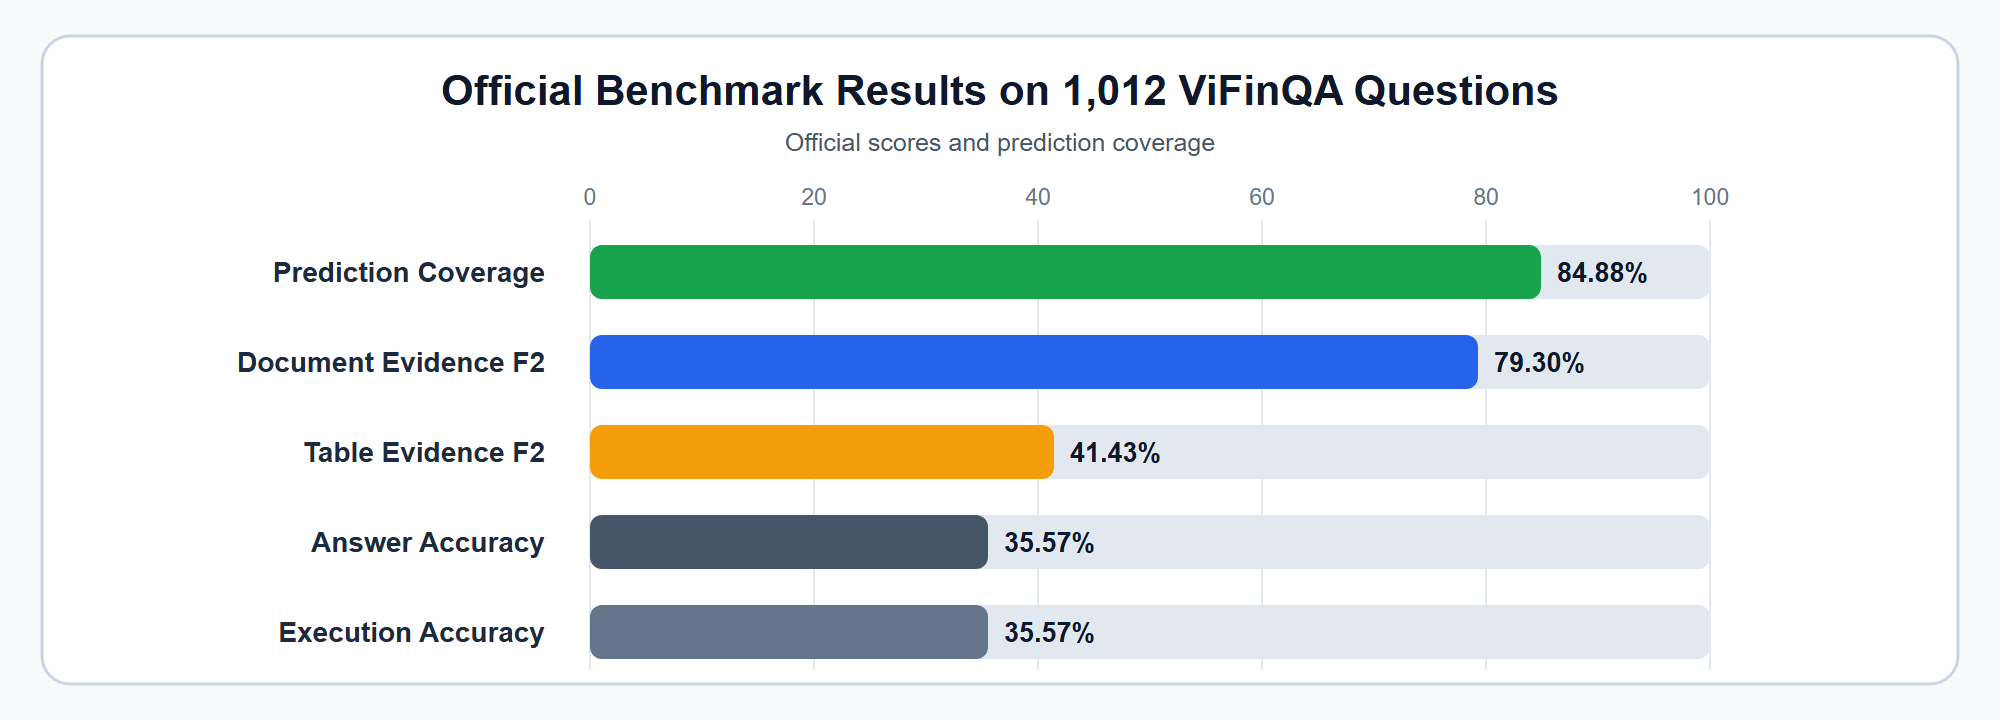
\includegraphics[width=0.94\textwidth]{figures/benchmark_results.png}
    \caption{Reported benchmark values for the ViFinQA evaluation set. Prediction Coverage is calculated from the prediction archive and is shown separately from the metrics produced by the official scorer.}
    \label{fig:benchmark_results}
\end{figure*}

In this submission, the document evidence metrics are higher than the table evidence metrics. Document evidence has an F2 Macro score of 79.30\% and an MRR at 5 score of 83.24\%. Table evidence has an F2 Macro score of 41.43\% and an MRR at 5 score of 48.85\%. These values describe a difference between the two evidence groups in the reported results. They do not by themselves identify the cause of that difference.

Answer Accuracy and Execution Accuracy are both reported as 35.57\%. The equality of these two values is recorded without an additional causal interpretation because the scoring archive does not include per question metric calculations. The prediction archive contains records for 859 of 1,012 questions, which gives a coverage value of 84.88\%. The other 153 questions do not have a prediction record. Coverage is reported as a separate property of the submission because the available files do not document how missing records are handled inside each official metric.

\subsection{Result Scope and Error Interpretation}

The available archives contain one scored system configuration. They do not contain a matched baseline or an ablation run on the same 1,012 questions. For this reason, this paper reports only the verified FinLens AI results and does not add unsupported comparisons.

The stored results show lower values for table evidence than for document evidence, together with incomplete prediction coverage. These observations can guide later analysis, but they are not sufficient to determine which pipeline stage caused each incorrect or missing answer. The archives do not provide a detailed failure label for each question. A more specific error analysis would require per question scoring details and failure records linked to the scored submission.

\section{Discussion \& Limitations}

\subsection{Discussion}
The current results describe how the main parts of FinLens operate as one product pipeline. Document evidence retrieval has an F2 Macro score of 79.30\%, while table evidence retrieval has an F2 Macro score of 41.43\%. This difference suggests that the system identifies relevant reports more consistently than the exact tables needed for calculation. However, the available results do not show which retrieval or selection step caused each error. This comparison is therefore presented as an observation rather than a causal conclusion.

FinLens separates document retrieval, table selection, context planning, code generation, validation, and sandbox execution. This structure allows a valid answer to be inspected together with its selected evidence and generated Pandas query. Before execution, the validation stage checks syntax, DataFrame aliases, units, rounding, and several calculation patterns. These checks support a more controlled execution process, but they do not confirm that the retrieved evidence or the financial interpretation is correct.

\subsection{Limitations}
The prediction archive contains results for 859 of 1,012 questions, which gives a prediction coverage of 84.88\%. Answer Accuracy and Execution Accuracy are both 35.57\%. These values show that the current implementation does not yet produce a valid and correct result for every question.

The system depends on the OCR extracted reports and on the table structure recovered during data preparation. Errors in headers, merged cells, labels, units, or report scope can affect later retrieval and calculation. The online pipeline also depends on the language model, Qdrant, the reranking service, and the E2B sandbox. A timeout or an unavailable service can prevent a prediction record from being produced.

The available evaluation files describe one scored system configuration. They do not include a matched baseline, an ablation study, or detailed scores for each question. The current results therefore describe the product as a whole and do not measure the separate contribution of each component. Further evaluation can examine failed questions, prediction coverage, table evidence selection, and numerical calculation as separate error groups.

\section{Conclusion}
FinLens is a Text to Pandas product for answering numerical questions over Vietnamese financial statements. It combines data preparation, table indexing, retrieval, table selection, context planning, code validation, sandbox execution, and answer traceability in one pipeline.

The evaluation uses all 1,012 questions in ViFinQA and contains prediction records for 859 questions. The results show a higher score for document evidence than for table evidence, while Answer Accuracy and Execution Accuracy are both 35.57\%. These results provide a current reference point for the product rather than a final measure of its performance. Further development can focus on producing valid records for more questions, selecting the correct tables more consistently, and improving the accuracy of the generated calculations.

\bibliographystyle{IEEEtran}
\bibliography{references}

\end{document}
